%% LyX 2.0.4 created this file.  For more info, see http://www.lyx.org/.
%% Do not edit unless you really know what you are doing.
\documentclass[oneside,dutch]{amsart}
\usepackage[T1]{fontenc}
\usepackage[latin9]{inputenc}
\usepackage[a4paper]{geometry}
\geometry{verbose,tmargin=3cm,bmargin=3cm,lmargin=2cm,rmargin=2cm}
\setlength{\parskip}{\smallskipamount}
\setlength{\parindent}{0pt}
\usepackage{amsthm}
\usepackage{graphicx}
\graphicspath{{Figures/}}

\makeatletter

%%%%%%%%%%%%%%%%%%%%%%%%%%%%%% LyX specific LaTeX commands.
%% Because html converters don't know tabularnewline
\providecommand{\tabularnewline}{\\}
%% A simple dot to overcome graphicx limitations
\newcommand{\lyxdot}{.}


%%%%%%%%%%%%%%%%%%%%%%%%%%%%%% Textclass specific LaTeX commands.
\numberwithin{equation}{section}
\numberwithin{figure}{section}

\makeatother

\usepackage{babel}
\begin{document}

\title{Relativiteit}


\author{N.G. Schultheiss}

\maketitle

\section{Inleiding}

In deze module wordt er uitgelegd hoe een natuurkundige gebeurtenis
door verschillende waarnemers wordt waargenomen. Iedere waarnemer
heeft een eigen assenstelsel en een eigen klok waarmee de gebeurtenis
wordt geobserveerd. De relatie tussen deze assenstelsels en klokken
wordt afgeleid.

Sommige grootheden zijn relatief en hangen af van de waarnemer en
daarmee het assenstelsel van de waarnemer. Andere grootheden hangen
niet af van het assenstelsel, deze worden invariant genoemd.

Uiteindelijk leidt dit tot de bekende formule van Einstein: $E=mc^{2}$.

Bestudeer de afleidingen goed, zodat je begrijpt hoe het maken van
een afleiding gaat.


\section{Lorentz en Poincar�}

Hendrik Antoon Lorentz is samen met Pieter Zeeman ��n van de vele
nederlandse Nobelprijswinnaars voor na\-tuur\-kunde. Je kent hem
onder andere van de Lorentzkracht $\mathbf{F}_{L}=l(\mathbf{I}\times\mathbf{B})$
of $F_{L}=BIlsin(\alpha)$. De Nobelprijs kreeg hij echter samen met
Zeeman voor het Zeeman-effect. Het Zeeman-effect beschrijft het effect
van magneten op de spin van deeltjes, hier komen we nog op terug.

Daarna wijdde Lorentz zich aan een eerste opzet van een relativiteitstheorie.
Voordat deze Lorentz transformatie werd toegepast, gebruikte men de
transformatie van Galile� om van een assenstelsel naar een assenstelsel'
te gaan:

\begin{equation}
\begin{array}{c}
x=x'+vt'\\
y=y'\\
z=z'\\
t=t'
\end{array}
\end{equation}


De grootheden zonder accent worden waargenomen door een waarnemer
in het assenstelsel zonder accent. De grootheden' met een accent worden
waargenomen door een waarnemer' in het assenstelsel' met accent%
\footnote{In de wiskunde wordt een accent ook wel gebruikt om de afgeleidde
van een functie aan te geven. Hier heeft dat niet zoveel zin, omdat
we dan niet weten of we de afgeleidde naar de tijd $t$ of de plaats
$(x,y,z)$ bedoelen. Om verwarring te voorkomen kunnen we bijvoorbeeld
de afgeleidde naar de tijd van de de functie $f(x,y,z,t)$ beter schrijven
als $\frac{df(x,y,z,t)}{dt}$.%
}.

Zoals je ziet verandert alleen het x-co�rdinaat. Galile� ging ervan
uit dat de tijd hetzelfde bleef voor alle assenstelsels. Volgens het
experiment van Michelson en Morley is de lichtsnelheid in alle assenstelsels
hetzelfde. De transformatie van een waarnemer naar een andere waarnemer
gaat dus niet meer volgens het paradigma van Galile�%
\footnote{Een paradigma is een idee dat de mensheid van de wereld heeft. Soms
blijkt dat dit idee niet juist is, dit noemt men een anomalie. Het
experiment van Michelson en Morley is dus te beschouwen als een anamolie
volgens het paradigma van Galile�.%
}. Het uitgangspunt wordt dus dat de lichtsnelheid langs de positieve
x-as in twee assenstelsels constant is:

\begin{equation}
\begin{array}{c}
c=\frac{\Delta x}{\Delta t}\\
c=\frac{\Delta x'}{\Delta t'}
\end{array}
\end{equation}


In beide stelsels kunnen we berekenen wanneer deze straal (op $t=0$
vanuit de oorsprong uitgezonden) op een plaats ($x$ of $x'$) wordt
waargenomen:

\begin{equation}
\begin{array}{c}
x=ct\\
x'=ct'
\end{array}
\end{equation}


\begin{equation}
\begin{array}{c}
x-ct=0\\
x'-ct'=0
\end{array}
\end{equation}


Omdat de tijdsduur voor beide assenstelsels kan verschillen kunnen
we voor beide stelsels schrijven:

\begin{equation}
x'-ct'=\lambda(x-ct)\label{eq:L1}
\end{equation}


Uiteraard geldt op gelijke wijze voor een lichtstraal langs de negatieve
x-as:

\begin{equation}
x'+ct'=\mu(x+ct)\label{eq:L2}
\end{equation}


Omdat beide formule's gelden, kunnen we kijken of $x'$ en $t'$ op
te lossen zijn. 

De som van \ref{eq:L1} en \ref{eq:L2} geeft:

\begin{equation}
x'-ct'+x'+ct'=\lambda(x-ct)+\mu(x+ct)
\end{equation}


\begin{equation}
2x'=(\lambda+\mu)x-(\lambda-\mu)ct
\end{equation}


\begin{equation}
x'=\frac{\lambda+\mu}{2}x-\frac{\lambda-\mu}{2}ct
\end{equation}


Het verschil geeft:

\begin{equation}
x'-ct'-(x'+ct')=\lambda(x-ct)-\mu(x+ct)
\end{equation}


\begin{equation}
-2ct'=(\lambda-\mu)x-(\lambda+\mu)ct
\end{equation}


\begin{equation}
ct'=-\frac{\lambda-\mu}{2}x+\frac{\lambda+\mu}{2}ct
\end{equation}


Deze formules zijn te vereenvoudigen als we twee nieuwe constanten
introduceren:

\begin{equation}
a=\frac{\lambda+\mu}{2}
\end{equation}


\begin{equation}
b=\frac{\lambda-\mu}{2}
\end{equation}


\begin{equation}
x'=ax-bct\label{eq:e15}
\end{equation}


\begin{equation}
ct'=-bx+act\label{eq:e16}
\end{equation}


\newpage{}

We kunnen nu bekijken hoe snel het stelsel' ten op zichte van het
stelsel beweegt. We nemen $x'=0$:

\begin{equation}
0=ax-bct
\end{equation}


\begin{equation}
v=\frac{x}{t}=\frac{bc}{a}
\end{equation}


\begin{equation}
\frac{v}{c}=\frac{b}{a}\label{eq:e19}
\end{equation}


Formule \ref{eq:e15} kan nu verder worden uitgewerkt:

\begin{equation}
x'=a\left(x-\frac{b}{a}ct\right)
\end{equation}


\begin{equation}
x'=a\left(x-\frac{v}{c}ct\right)
\end{equation}


Formule \ref{eq:e16} is ook te herschrijven:

\begin{equation}
ct=\frac{ct'}{a}+\frac{bx}{a}
\end{equation}


\begin{equation}
ct=\frac{ct'}{a}+\frac{vx}{c}
\end{equation}


Substitutie geeft:

\begin{equation}
x'=a\left(x-\frac{v}{c}\left(\frac{ct'}{a}+\frac{vx}{c}\right)\right)
\end{equation}


\begin{equation}
x'=a\left(1-\left(\frac{v}{c}\right)^{2}\right)x-a\frac{v}{c}\frac{ct'}{a}
\end{equation}


\begin{equation}
x'=a\left(1-\left(\frac{v}{c}\right)^{2}\right)x-vt'\label{eq:e26}
\end{equation}


We nemen de klok zo dat $t=t'=0$. Uit formule \ref{eq:e15} volgt
dan:

\begin{equation}
x'=ax
\end{equation}


Vanuit het stelsel neemt men een lengte van 1 in het stelsel' waar
als:

\begin{equation}
x=\frac{1}{a}
\end{equation}


Uit formule \ref{eq:e26} volgt nu:

\begin{equation}
x'=a\left(1-\left(\frac{v}{c}\right)^{2}\right)x
\end{equation}


Vanuit het stelsel' neemt men een lengte van 1 in het stelsel waar
als:

\begin{equation}
x'=a\left(1-\left(\frac{v}{c}\right)^{2}\right)
\end{equation}


Omdat we in beide stelsels een eenheidsmaat hetzelfde waarnemen in
het andere stelsel geldt:

\begin{equation}
x=x'
\end{equation}


\begin{equation}
\frac{1}{a}=a\left(1-\left(\frac{v}{c}\right)^{2}\right)
\end{equation}


\begin{equation}
a=\frac{1}{\sqrt{1-\left(\frac{v}{c}\right)^{2}}}
\end{equation}


Uit formule \ref{eq:e19} volgt:

\begin{equation}
b=\frac{\frac{v}{c}}{\sqrt{1-\left(\frac{v}{c}\right)^{2}}}
\end{equation}


Invullen in \ref{eq:e15} en \ref{eq:e16} geeft de transformatie
voor plaats en tijd:

\begin{equation}
x'=\frac{x-vt}{\sqrt{1-\left(\frac{v}{c}\right)^{2}}}
\end{equation}


\begin{equation}
t'=\frac{t-\frac{v}{c^{2}}x}{\sqrt{1-\left(\frac{v}{c}\right)^{2}}}
\end{equation}


De verandering van de plaats verschilt van de Galile� transformaties.
De verandering is als een nieuwe constante te schrijven, de Lorentzconstante:

\begin{equation}
\gamma=\frac{1}{\sqrt{1-\left(\frac{v}{c}\right)^{2}}}
\end{equation}


Lorentz hing het idee van ``aether'' aan en had zelf moeite om de
door hem afgeleidde formules te aanvaarden. In een briefwisseling
met Lorentz opperde Jules Henri Poincar� verder het idee dat de ruimte
als vierdimensionaal voor te stellen is. De Lorentztransformaties
beschrijven hoe deze vierdimensionale ruimte wordt vervormd als men
deze vanuit het stelsel van ene waarnemer en vanuit het stelsel van
de andere waarnemer' bekijkt. Als men de tijd imaginair%
\footnote{Meestal wordt een imaginair getal aangeduidt met $i$. Dit is ook
te defini�ren met $i=\sqrt{-1}$.%
} neemt, blijft de lengte van de vectoren in deze vierdimensionale
ruimte gelijk en is te schrijven met:

\begin{equation}
x^{2}+y^{2}+z^{2}-\left(ct\right)^{2}=x'^{2}+y'^{2}+z'^{2}-\left(ct'\right)^{2}
\end{equation}


Poincar� werkte ook aan de effecten van de terugstoot van bijvoorbeeld
de door Madame Curie gevonden straling. Voor de publicatie van Einstein
betreffende de speciale relativiteitstheorie publiceerde hij: 'Poincar�,
H. (1905), Sur la dynamique de l'�lectron'. In 1906 schreef hij een
tweede artikel met dezelfde titel%
\footnote{Beiden zijn op internet te vinden. Ik behandel de besproken wiskunde
hier niet. Het is inderdaad heel veel werk en het heeft weinig resultaat.%
}. Hierna stopte Poincar� (helaas) met de vierdimensionale ruimte omdat
hij het te veel werk met te weinig resultaat vond.


\section{\label{sec:Invarianten}Invarianten}

Hiervoor hebben we gezien dat diverse grootheden kunnen veranderen
als we van assenstelsel wisselen. Sommige grootheden doen dit niet,
deze worden ``invariant'' genoemd. Zoals Michelson en Morley experimenteel
bepaalden, is de lichtsnelheid een invariant.

We kunnen de toestand van een object bijvoorbeeld beschrijven met
de plaatsvector en de tijd. Omdat alles relatief is, zijn de plaatsvector
en de tijd dit natuurlijk ook. Een andere manier, die ook direct voor
botsingen te gebruiken is, is een beschrijving met impuls en energie.
Zowel de impuls als de plaats kennen 3 richtingen: \emph{x}, \emph{y}
en \emph{z}. De tijd is volgens Poincar� en Minkowsky (in het geval
van de plaats) op te vatten als een $4^{e}$ richting. In het geval
van de impuls geldt dit ook voor de energie.

De toestand van het object is dus te beschouwen als een vierdimensionale
vector of 4-vector. De vier componenten van een impuls/energievector
kunnen op de volgende wijze van een assenstelsel naar een assenstelsel'
dat in de x-richting beweegt wisselen:

\begin{equation}
\begin{array}{c}
p_{x'}=\gamma\left(p_{x}-\beta\frac{E}{c}\right)\\
p_{y'}=p_{y}\\
p_{z'}=p_{z}\\
\frac{E'}{c}=\gamma\left(\frac{E}{c}-\beta p_{x}\right)
\end{array}\label{eq:e6.1}
\end{equation}


In deze set formules zien we de variabelen $\beta$ en $\gamma$.
De variabele $\beta$ geeft aan hoe snel de assenstelsels ten opzichte
van elkaar bewegen: $\beta=\frac{v}{c}$. Als we met deze formule
terug willen naar het eerste assenstelsel nemen we $\beta$ negatief.
De Lorentzconstante $\gamma$ is nu te schrijven als: $\gamma=\frac{1}{\sqrt{1-\beta^{2}}}$%
\footnote{Uiteraard geldt: $\beta^{2}=\left(-\beta\right)^{2}$. De transformatie
van het ene naar het andere stelsel en terug is dus met dezelfde Lorentzconstante
$\gamma$ te beschrijven.%
}.

De lengte van deze 4-vector is met de stelling van Pythagoras te bepalen.
Als we de tijd- of de energie-component imaginair nemen, dan blijkt
deze vector ook invariant te zijn. Als men de tijd of de energie-component
dan kwadradeert, wordt het resultaat negatief. Blijkbaar geldt dus:

\begin{equation}
p_{x'}^{2}+p_{y'}^{2}+p_{z'}^{2}-\left(\frac{E'}{c}\right)^{2}=p_{x}^{2}+p_{y}^{2}+p_{z}^{2}-\left(\frac{E}{c}\right)^{2}
\end{equation}


Dit is natuurlijk wiskundig te controleren. Substitutie van de formules
van \ref{eq:e6.1} geeft de te bewijzen bewering:

\begin{equation}
\left(\gamma\left(p_{x}-\beta\frac{E}{c}\right)\right)^{2}+p_{y}^{2}+p_{z}^{2}-\left(\gamma\left(\frac{E}{c}-\beta p_{x}\right)\right)^{2}=p_{x}^{2}+p_{y}^{2}+p_{z}^{2}-\left(\frac{E}{c}\right)^{2}\Rightarrow
\end{equation}


\begin{equation}
\left(\gamma\left(p_{x}-\beta\frac{E}{c}\right)\right)^{2}-\left(\gamma\left(\frac{E}{c}-\beta p_{x}\right)\right)^{2}=p_{x}^{2}-\left(\frac{E}{c}\right)^{2}\Rightarrow
\end{equation}


\begin{equation}
\gamma^{2}\left(p_{x}^{2}-2p_{x}\beta\frac{E}{c}+\beta^{2}\left(\frac{E}{c}\right)^{2}\right)-\gamma^{2}\left(\left(\frac{E}{c}\right)^{2}-2p_{x}\beta\frac{E}{c}+\beta^{2}p_{x}^{2}\right)=p_{x}^{2}-\left(\frac{E}{c}\right)^{2}\Rightarrow
\end{equation}


\begin{equation}
\gamma^{2}p_{x}^{2}-2\gamma^{2}p_{x}\beta\frac{E}{c}+\gamma^{2}\beta^{2}\left(\frac{E}{c}\right)^{2}-\gamma^{2}\left(\frac{E}{c}\right)^{2}+2\gamma^{2}p_{x}\beta\frac{E}{c}-\gamma^{2}\beta^{2}p_{x}^{2}=p_{x}^{2}-\left(\frac{E}{c}\right)^{2}\Rightarrow
\end{equation}


\begin{equation}
\gamma^{2}p_{x}^{2}-\gamma^{2}\beta^{2}p_{x}^{2}-2\gamma^{2}p_{x}\beta\frac{E}{c}+2\gamma^{2}p_{x}\beta\frac{E}{c}+\gamma^{2}\beta^{2}\left(\frac{E}{c}\right)^{2}-\gamma^{2}\left(\frac{E}{c}\right)^{2}=p_{x}^{2}-\left(\frac{E}{c}\right)^{2}\Rightarrow
\end{equation}


\begin{equation}
\gamma^{2}\left(1-\beta^{2}\right)p_{x}^{2}+\gamma^{2}\left(\beta^{2}-1\right)\left(\frac{E}{c}\right)^{2}=p_{x}^{2}-\left(\frac{E}{c}\right)^{2}\Rightarrow
\end{equation}


\begin{equation}
\frac{1-\beta^{2}}{1-\beta^{2}}p_{x}^{2}+\frac{\beta^{2}-1}{1-\beta^{2}}\left(\frac{E}{c}\right)^{2}=p_{x}^{2}-\left(\frac{E}{c}\right)^{2}\Rightarrow
\end{equation}


\begin{equation}
p_{x}^{2}-\left(\frac{E}{c}\right)^{2}=p_{x}^{2}-\left(\frac{E}{c}\right)^{2}
\end{equation}


Waarmee bewezen is dat de lengte van deze 4-vector een invariant is.

Het blijkt dat de lengte van deze 4-vector te koppelen is aan een
andere invariant, de (rust-)massa. In hoofdstuk  \ref{sec:Einstein-en-Minkowski}
zien we hoe Einstein afleidde dat als $p_{x}=\gamma mv$, $E=\gamma mc^{2}$
wordt. Invullen geeft:

\begin{equation}
p_{x}^{2}-\left(\frac{E}{c}\right)^{2}=\left(m\gamma v\right)^{2}-\left(\frac{m\gamma c^{2}}{c}\right)^{2}=m^{2}c^{2}\gamma^{2}\left(\left(\frac{v}{c}\right)^{2}-1\right)=m^{2}c^{2}\frac{\beta^{2}-1}{1-\beta^{2}}
\end{equation}


\begin{equation}
m^{2}c^{2}=\left(\frac{E}{c}\right)^{2}-p^{2}\label{eq:e12}
\end{equation}


Met deze formule is ook direct de impuls van fotonen te bepalen. Omdat
een foton geen (rust-)massa heeft, kan men afleiden dat $p_{foton}=\frac{E_{foton}}{c}$.
Of volgens Planck: $p_{foton}=\frac{h\nu}{c}$.

Verder valt op dat, als we onze eenheden zo nemen dat alles in lichtsnelheden
en seconden wordt uitgedrukt%
\footnote{Deze eenheden staan bekend als Natural Units (NU) en kunnen op verschillende
wijzen worden gedefini�erd. Met Heaviside-Lorentz Units wordt de lichtsnelheid
ook 1 omdat men $\varepsilon_{0}$ en $\mu_{0}$ op 1 stelt. Omdat
$c^{2}=\frac{1}{\varepsilon_{0}\mu_{0}}$ is, wordt $c=1$.%
}, formule \ref{eq:e12} kan worden geschreven als:

\begin{equation}
m=\sqrt{E^{2}-p^{2}}
\end{equation}


Dit wisselen van eenheden wordt vaak gebruikt om de wiskunde van een
natuurkundig probleem overzichtelijker te maken. Een andere methode
is om de variabelen dimensieloos of ``zonder eenheden'' te maken.
Voorbeelden hiervan zijn de variabelen $\beta$ en $\gamma$.


\section{\label{sec:Einstein-en-Minkowski}Einstein en Minkowski}

Albert Einstein onderzocht de terugstoot van licht met een gedachte
experiment en kwam daarmee op de formule $E=mc^{2}$. Hij ging uit
van een gesloten doos (in rust) met een lengte $l$ en een massa $m_{doos}$.
Aan de linkerkant zenden we een foton naar rechts, even later wordt
dit aan de rechterkant geabsorbeerd. Hiervoor hebben we gezien dat
de impuls van het foton te schrijven als:

\begin{equation}
p_{foton}=\frac{E_{foton}}{c}
\end{equation}


Verder geldt:

\begin{equation}
p_{doos}=m_{doos}v_{doos}
\end{equation}


De snelheid van de doos is te vinden door de verplaatsing van de doos
te delen door de tijd dat het foton bestaat:

\begin{equation}
p_{doos}=m_{doos}\frac{\Delta x_{doos}}{\Delta t}
\end{equation}


Uiteraard geldt de wet van behoud van impuls, omdat de doos in het
begin stilstond geldt:

\begin{equation}
m_{doos}\frac{\Delta x_{doos}}{\Delta t}+\frac{E_{foton}}{c}=0
\end{equation}


We weten dat het foton met de lichtsnelheid reist, de doos verplaatst
zich dus gedurende $\Delta t=\frac{l}{c}$ seconden.

\begin{equation}
m_{doos}\frac{\Delta x_{doos}}{l}+\frac{E_{foton}}{c^{2}}=0\label{eq:e5}
\end{equation}


Als we weten hoever de doos zich verplaatst is de formule opgelost.
We introduceren een nieuwe grootheid $m_{foton}$, omdat fotonen met
de lichtsnelheid bewegen is deze impuls ook te schrijven als $m_{foton}c$.
De wet van behoud van impuls blijft gelden%
\footnote{Hier is iets vreemds aan de hand, het foton beweegt natuurlijk slechts
over de lengte van de doos min de verplaatsing van de doos. Als we
de massa van de doos heel groot ten opzichte van die van het foton
nemen, mag deze verwaarlozing echter wel. Hoe zit het trouwens met
$\Delta t$?%
}:

\begin{equation}
m_{foton}c+m_{doos}v_{doos}=0
\end{equation}


\begin{equation}
m_{foton}c\Delta t+m_{doos}v_{doos}\Delta t=0
\end{equation}


\begin{equation}
m_{foton}l+m_{doos}\Delta x_{doos}=0
\end{equation}


\begin{equation}
m_{doos}\frac{\Delta x_{doos}}{l}+m_{foton}=0
\end{equation}


Substitutie in formule \ref{eq:e5} geeft:

\begin{equation}
m_{foton}=\frac{E_{foton}}{c^{2}}
\end{equation}


Generaliseren geeft de bekende formule:

\begin{equation}
E=mc^{2}
\end{equation}


Als in een voorwerp energie wordt gestopt, neemt de massa van dat
voorwerp volgens Einstein dus toe. Omdat we in hoofdstuk \ref{sec:Invarianten}
hebben gevonden dat de lengte van een 4-vector en daarmee de (rust)massa
$m$ invariant is, nemen we voor de massa een nieuwe variabele $M$:

\begin{equation}
E=Mc^{2}=\alpha mc^{2}
\end{equation}


De waargenomen massa $M$ is dus een factor $\alpha$ groter dan de
rustmassa $m$%
\footnote{In de literatuur wordt voor de rustmassa ook vaak $m_{0}$ gebruikt.
De massa wordt dan niet met $M$ maar met $m$ aangeduidt.%
}. We kunnen nu ook de impuls van dit deeltje uitrekenen:

\begin{equation}
p=Mv=\alpha mv
\end{equation}


Dit is in te vullen in formule \ref{eq:e12}:

\begin{equation}
m^{2}c^{2}=\left(\frac{\alpha mc^{2}}{c}\right)^{2}-\left(\alpha mv\right)^{2}
\end{equation}


\begin{equation}
m^{2}=\alpha^{2}m^{2}\left(1-\left(\frac{v}{c}\right)^{2}\right)
\end{equation}


\begin{equation}
\alpha^{2}=\frac{1}{1-\left(\frac{v}{c}\right)^{2}}
\end{equation}


\begin{equation}
\alpha=\frac{1}{\sqrt{1-\left(\frac{v}{c}\right)^{2}}}
\end{equation}


Het blijkt dus dat de constante $\alpha$ gelijk is aan de Lorentzconstante
$\gamma$. De waargenomen massa kan dus ook worden geschreven als
$M=\gamma m$. De energie kan dus ook worden geschreven als:

\begin{equation}
E=\gamma mc^{2}
\end{equation}


Zoals te zien is, heeft een voorwerp met een snelheid van 0m/s al
energie. Onze klassieke formule voor de bewe\-gingsenergie geeft
dus eigenlijk de e\-ner\-giever\-andering: $\Delta E=\frac{1}{2}mv^{2}$.
In tabel 1 is te zien welke gevolgen dit voor verschillende snelheden
heeft. Het valt op dat bij lage snelheden ten opzichte van de lichtsnelheid
beide modellen dezelfde waarden geven. Dit is natuurlijk wel te verwachten.
De klassieke natuurkunde die door mensen als Galile�, Huygens, Keppler
en Newton is vormgegeven, nam geen verschijnselen waar die in de buurt
van de lichtsnelheid kwamen. Met de klassieke wetten zijn de verschijnselen
die wel waargenomen werden goed te verklaren. Bij $0.1c$ is de afwijking
minder dan 1\%, de snelheid is dan dus 30000km/s. Deze snelheid is
vrij hoog in vergelijking met de snelheid van een paard.

\begin{table}[h]
\begin{centering}
\begin{tabular}{|c|c|c|}
\hline 
$v$  & $E_{Einstein}$ (J) & $\Delta E_{Klassiek}$ (J)\tabularnewline
\hline 
\hline 
$0c$ & $mc^{2}$ & $0$\tabularnewline
\hline 
$0,1c$ & $mc^{2}+0,005mc^{2}$ & $0,005mc^{2}$\tabularnewline
\hline 
$0,2c$ & $mc^{2}+0,021mc^{2}$ & $0,020mc^{2}$\tabularnewline
\hline 
$0,3c$ & $mc^{2}+0,048mc^{2}$ & $0,045mc^{2}$\tabularnewline
\hline 
$0,4c$ & $mc^{2}+0,091mc^{2}$ & $0,080mc^{2}$\tabularnewline
\hline 
$0,5c$ & $mc^{2}+0,155mc^{2}$ & $0,125mc^{2}$\tabularnewline
\hline 
$0,6c$ & $mc^{2}+0,250mc^{2}$ & $0,180mc^{2}$\tabularnewline
\hline 
$0,7c$ & $mc^{2}+0,400mc^{2}$ & $0,245mc^{2}$\tabularnewline
\hline 
$0,8c$ & $mc^{2}+0,667mc^{2}$ & $0,320mc^{2}$\tabularnewline
\hline 
$0,9c$ & $mc^{2}+1,294mc^{2}$ & $0,405mc^{2}$\tabularnewline
\hline 
$1,0c$ & $\infty$ & $0,500mc^{2}$\tabularnewline
\hline 
\end{tabular}\\
\medskip{}

\par\end{centering}

\caption{Vergelijking van de energie volgens Einstein met de bewegingsenergie}
\end{table}


\begin{figure}[h]
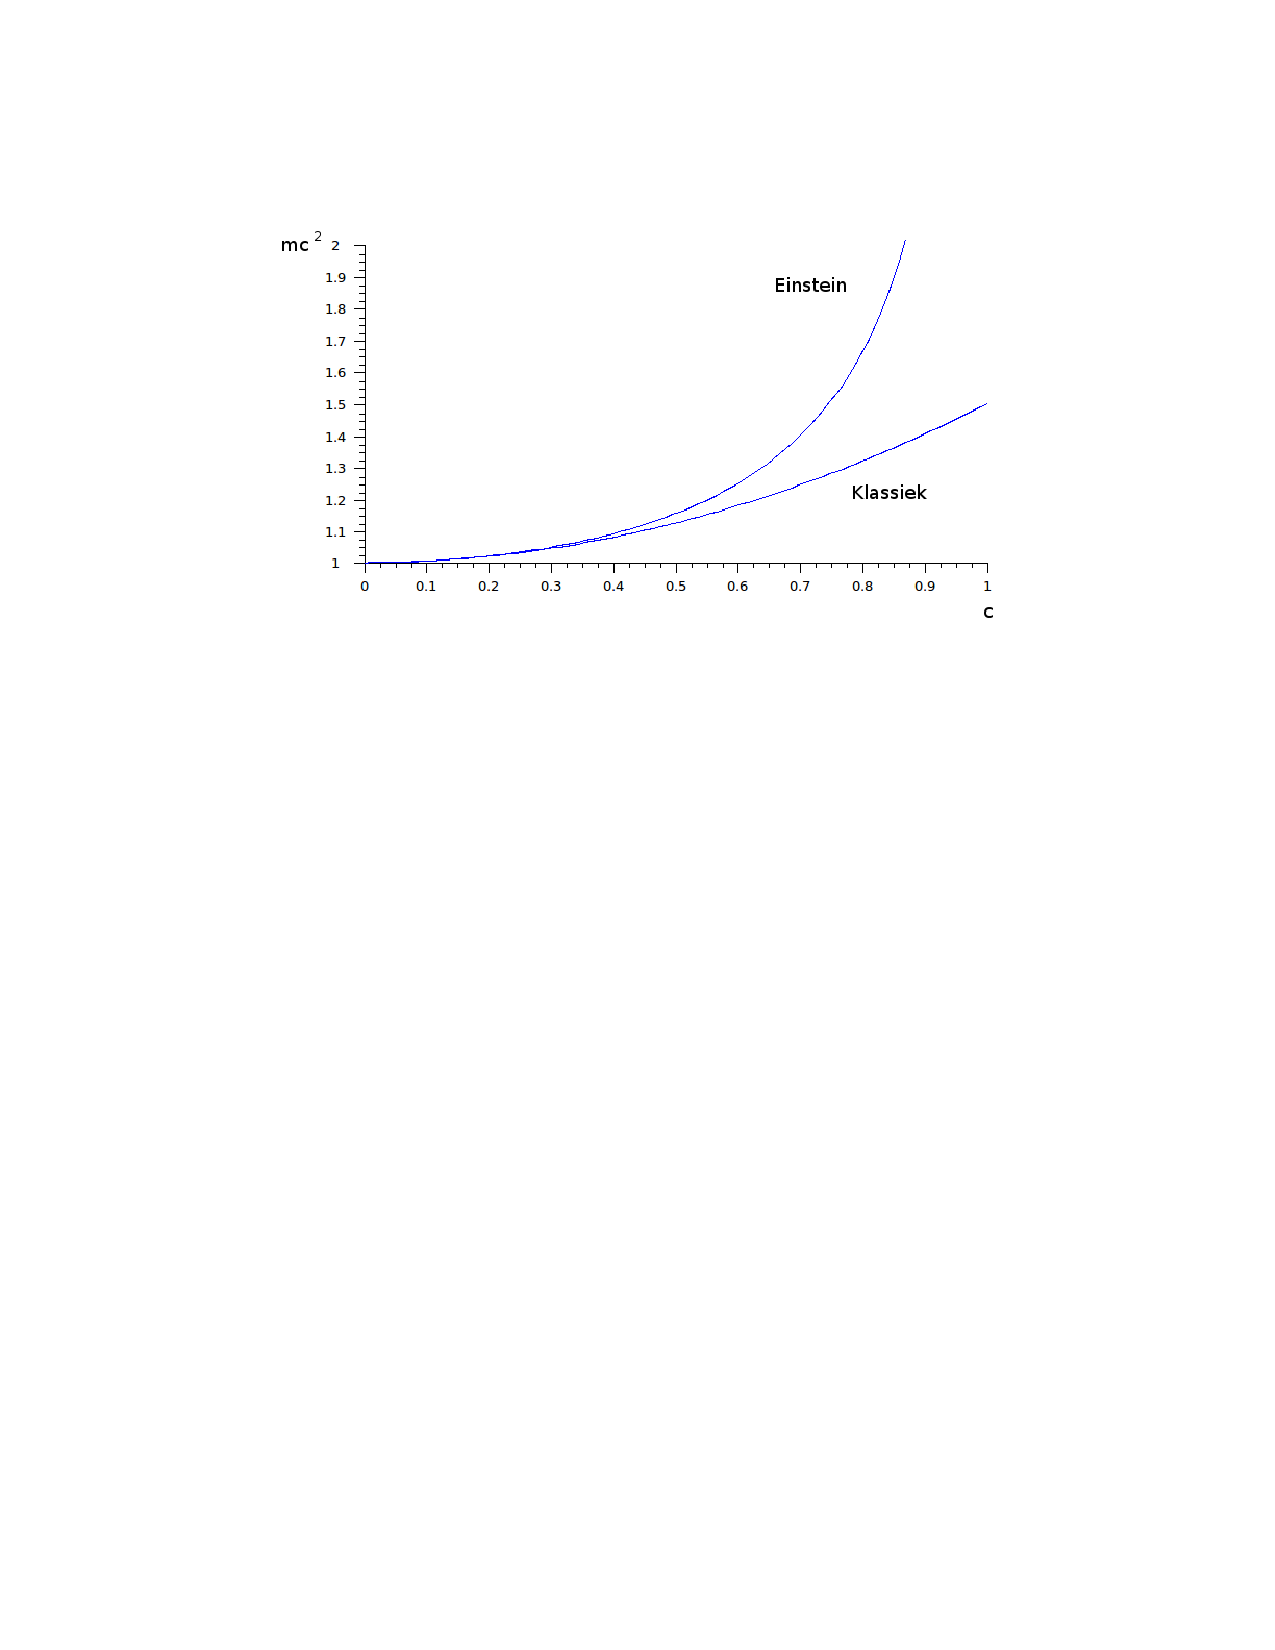
\includegraphics[scale=1]{einstein}

\caption{De energie als functie van $c$ tegen de energie volgens Einstein
en de bewegingsenergie}
\end{figure}


Voor lage snelheden kunnen we de werkelijkheid dus goed benaderen
met klassieke natuurkunde. Bij hoge snelheden gaat dit helaas niet
meer. Omdat de snelheid van een massa nooit tot de lichtsnelheid kan
komen, kunnen we in dit geval beter zeggen dat de energie bij benadering
wordt gebruikt voor de massatoename van een deeltje. Een direct logisch
gevolg is dat deeltjes die zich met de lichtsnelheid verplaatsen geen
massa hebben.

Met de wetten van behoud van energie en impuls lijkt het er op dat
we nu botsingen van deeltjes met snelheden in de buurt van de lichtsnelheid
kunnen berekenen.

Albert Einstein kreeg in Zurich wiskunde van Hermann Minkowski. Minkowski
hield zich onder andere bezig met meerdimensionale wiskundige problemen.
Minkowski werkte de idee�n die door Poincar� waren geopperd verder
uit tot de Minkowski-ruimte.

In 1915 werd de speciale relativiteitstheorie door Einstein uitgebreid
met de algemene relativiteitstheorie. De zwaartekracht wordt hierin
verklaard door de kromming van de ruimte.


\paragraph*{Opdracht:}

\emph{In de hoofdstukken ``Invarianten'' en ``Einstein en Minkovsky''
lopen we het risico dat er een kringredene\-ring}%
\footnote{Een kringredenering ontstaat als we een aanname voor redenering 1
gebruiken om redenering 2 te bewijzen en daarna een aanname voor redenering
2 gebruiken om redenering 1 te bewijzen. %
}\emph{ plaatsvindt. Welk risico is dit en is dit een probleem? }
\end{document}
